\documentclass[12pt]{article}
\usepackage[osf]{mathpazo}
\usepackage{ms}
\usepackage[numbers]{natbib}
\usepackage{lineno}
\usepackage{graphicx}
\usepackage{caption}
\modulolinenumbers[5]
\linenumbers

\makeatletter
\renewcommand{\@biblabel}[1]{\quad#1.}
\makeatother

\title{How much of the world is woody?}
\author{
Richard G. FitzJohn$^{*,\dag,1,2}$, Matthew W. Pennell$^{*,3,4}$, Amy E. Zanne$^{5,6}$,\\ Peter F. Stevens$^{7}$, David C. Tank$^{3,8}$, William K. Cornwell$^{9}$
}
\date{}
\affiliation{\noindent
$^*$ These authors contributed equally\\
$^\dag$ To whom correspondence should be addressed\\
$^1$ Biodiversity Research Centre and Department of Zoology,
University of British Columbia, Vancouver, BC V6G 1Z4, Canada \\
$^2$ Department of Biological Sciences, Macquarie University, Sydney, NSW 2109, Australia \\
$^3$ Institute for Bioinformatics and Evolutionary Studies, University of Idaho, Moscow, ID 83844, U.S.A.\\
$^4$ National Evolutionary Synthesis Center, Durham, NC 27705, U.S.A.\\
$^5$ Department of Biological Sciences, George Washington University, Washington, D.C. 20052, U.S.A.\\
$^6$ Center for Conservation and Sustainable Development, Missouri Botanical Garden, St. Louis, MO, 63121, USA \\
$^7$Department of Biology, University of Missouri, St. Louis, MO 63166, U.S.A.\\
$^8$ Department of Forest, Rangeland, and Fire Sciences and Stillinger Herbarium, College of Natural Resources, University of Idaho, Moscow, ID 83844, U.S.A.\\
$^9$ Department of Systems Ecology, VU University, 1081 HV Amsterdam, The Netherlands
}
\runninghead{How much of the world is woody?}
\keywords{Database, Herbaceousness, Macroecology, Woodiness}

\begin{document}
\mstitlepage
\parindent=1.5em
\addtolength{\parskip}{.3em}

\begin{abstract}
  The question posed by the title of this paper is a basic one; it is
  surprising that the answer is not known given that the
  woody/herbaceous divide is perhaps the most fundamental axis of
  functional diversity among plants.
  % 
  We informally surveyed a broad community of biologists to
  determine whether a consensus answer to our question existed ---
  even if not documented in the peer-reviewed literature.  No such
  consensus existed, with estimates ranging from 1\% to 90\% (mean:
  31.7\%).
  % 
  With a database of woodiness for 49,064 species of vascular plants
  we estimated the status of the remaining
  %
  235,668 species using two randomisation approaches.  We estimated
  the proportion woodiness among the world's vascular plants to be
  between 45\% and 48\%.
  %
  This estimate is larger than 81\% of the estimates in our survey,
  most of which substantially underestimated the proportion of the
  world's flora that was woody.  The results of our survey highlight
  that global datasets can show patterns at odds with conventional
  wisdom.
\end{abstract}

\vfill
\paragraph{Keywords:} \thekeywords

\newpage
\section{Introduction}

The distinction between a woody and non-woody growth-form is
probably the most profound contrast among terrestrial plants and
ecosystems: the difference between a forest and a grassland is the
presence or absence of wood. The recognition of the fundamental
importance of this divide dates back at least to \textit{Enquiry into
  Plants} by Theophrastus of Eresus (371 -- 287 BC), a student of
Plato and Aristotle, who began his investigation into plant form and
function by classifying the hundreds of plants in his garden into
woody and herbaceous categories \citep{theophrastus1916enquiry}.

The last two thousand years of research into wood since Theophrastus
classified his garden have uncovered its origin in the early Devonian
($\sim$~400 Mya) \citep{gerrienne2011simple}; that prevalence of
woodiness varies with climate \citep{Molesheihgt}; that wood has been
lost many times in diverse groups, both extant and extinct
\citep{judd1994}; and that many different forms of pseudo-woody growth
habit have appeared across groups that have lost true woodiness or
diverged before true woodiness evolved \citep{Cornwellwood}.  We know
about its mechanical properties and developmental pathways, its
patterns of decomposition and their effects on ecosystem function
\citep{Cornwellwood}, and that woody and herbaceous species have
markedly different rates of molecular evolution \citep{SmithDonoghue}.
%
However, we have no idea about what proportion of species are actually
woody.

With the rise of bioinformatics, the similar biodiversity question of
``how many species are there on earth'' has been approached with a
variety of different methods \citep{may1988many,erwin1991many,
  stork1993many, joppa2010, costello2011, mora2011plos}.  These
statistical estimates are improved, narrowing in most recently on a
number around 8.7 million species with approximately 300,000 of those
plants \citep{mora2011plos}, although considerable variation still
exists among estimates \citep{costello2011}.

We aim to use similar tools to re-ask Theophrastus' 2000 year old
question at a global scale: how many of the world's plant species are
woody?
%
We felt that such a basic question would be essentially known.
%
However, discussions among our ``Tempo and Mode of Plant Trait
Evolution'' NESCent working group revealed a wide range of opinions
and very little published research, with the exception of an almost
100-year old paper \citep{sinnott1915evolution}.
%
Because of this, we took the unconventional approach of coupling our
analysis with with an informal survey in which we asked our question
to the broader community of botanists and other biologists.
% 
The tremendous variety of answers in response suggests that this
fundamental aspect of plant functional diversity is surprisingly
poorly understood.

\section{Methods and Materials}

\subsection{Survey}

We first investigated whether a general consensus among biologists
existed.  The motivation for this was to determine whether a consensus
answer existed --- even if not formalised in the literature --- and if
so, whether it was consistent with the data.
% 
In a similar study, botanical experts largely agreed with the
model--estimated number of species in several Angiosperm groups
\citep{joppa2010}, and we were interested in whether there was similar
anecdotal knowledge for the relative prevalence of this key trait.
%
We created an English-language survey asking for an estimate of the
percentage of species that are woody according to the above
definition.  We also asked respondents to indicate their level of
familiarity with plants, level of formal training, and the country in
which they received their training (see supplementary material Figure
\ref{fig:survey-text} for details).
%
We distributed the survey to the community via several electronic
mailing lists with wide circulation among biologists: \emph{EvolDir},
\emph{ECOLOG}, \emph{\mbox{r-sig-phylo}}, \emph{Taxacom},
\emph{Herbaria}, as well as local lists. We also posted links on the
social-networking platforms \textsc{google+}, \textsc{twitter} and
\textsc{facebook} to reach a broad audience.
%
In order to increase representation of survey responses from Latin
America, we translated the survey into Portuguese (thanks to Rafael
Maia) and distributed it to Brazilian biology
\textsc{facebook} groups and university mailing lists.

To analyse the survey data, we used linear regression on
logit-transformed percent woodiness as (for discussion as to why we
used logit--transform, see ref \citep{wartonarcsine}) and treated the
self-reported level of botanical familiarity and education as factors.
We converted country of training to coarse latitude using shapefiles
from the GBIF dataportal\\
(\texttt{http://code.google.com/p/gbif-dataportal/wiki/ConfiguringGeoserver}),
and converted these into ``tropical'' and ``temperate'' using an
absolute latitude of 23$^\circ$~26$^\prime$.  All analyses were
conducted with R version 2.15.1 \citep{R}.

\subsection{Dataset}

We used a recently assembled database with growth-form data for 49,064
vascular plant species, which is the largest such database assembled
to date (see ref \citep{Zanne}). The core of the woodiness dataset
came from Kew Royal Botanic Gardens dataset on growth form
\citep{Kew}.  We reduced the original 103 growth form categories to a
binary classification following a ``functional'' definition of
woodiness as a plant with a ``prominent, persistent above-ground
stem''.  Fifty seven of the 103 categories provided enough information
to classify species as either woody or herbaceous according to our
definition (see Table \ref{tab:kew} for specific decisions).  In
addition, several smaller datasets were added according to the same
categorisation \citep{Zanne}.  Note that in addition to species
producing true wood (i.e., consisting of secondary xylem), this
definition classifies, among other groups, palms, tree ferns, and
bamboo as woody.

Taxonomically, we included vascular plants (i.e., lycopods, ferns,
gymnosperms, and angiosperms).
%
Because the effort to organise plant taxonomy, especially synonymy, is
on-going, there was uncertainty regarding the status of many of these
plant names.  
%
To bring species binomials to a common taxonomy among datasets, names
were matched against accepted names in the Plant List
\citep{ThePlantList}.  Any binomials not found in this list were
matched against the International Plant Name Index
(http://www.ipni.org/) and Tropicos (http://www.tropicos.org/);
potential synonymy in binomials arising from the three lists was
investigated using the Plant List tools \citep{ThePlantList}.  
%
Binomials remaining unmatched were compared first to the Plant List
and if needed to IPNI with an approximate matching algorithm to allow
for misspellings, followed by manual verification.

Theophrastus both recognised the fundamental importance of the
distinction between woody and herbaceous plants, and that this
distinction is in some cases difficult to make.  There are a number of
species which are intermediate in form \citep{beaulieuHiddenRates}; in
this dataset 633 species (1.3\%) were coded as variable and were
excluded from our analysis.
%
Our final database contained 37,488 records with both information on
woodiness and documented taxonomy---15,657 herbs and 21,831 woody
species.  This included records from all plant orders currently
accepted by APG-III \citep{APG3} along with the ferns taxonomy from
ref \cite{apweb}.
% sum(dat.g$K) # known species
% sum(dat.g$H) # herbs
% sum(dat.g$W) # woody species

% WKC: compare family sampling to total number of families? Somehow
% show the dataset is comprehensive?

\subsection{Estimating the percentage of species that are woody}

To estimate the percentage of species that are woody, we cannot simply
use the fraction of species within our trait database (21,831 of
37,488 = 58\%) as these records represent a biased sample of vascular
plants.
% sum(dat.g$W) # woody
% sum(dat.g$K) # known
% sum(dat.g$W) / sum(dat.g$K) # fraction
For example, most Orchidaceae are probably herbaceous; we have only
two records of woodiness among the 1,574 species for which we have
data.
% i.orc <- dat.g$family == "Orchidaceae"
% sum(dat.g$K[i.orc]) # known Orchidaceae
% sum(dat.g$W[i.orc]) # woody Orchidaceae
However, the fraction of Orchidaceae with known data (1,574 of 27,104
= 6\%)
% sum(dat.g$K[i.orc]) # known Orchidaceae
% sum(dat.g$N[i.orc]) # number of Orchidaceae
% sum(dat.g$K[i.orc]) / sum(dat.g$N[i.orc]) # knowledge rate of Orchidaceae
is much lower than the overall rate of knowledge for all vascular
plants (36,238 of 274,141 = 13\%), which will upwardly bias the global
estimate of woodiness.
% sum(dat.g$K) # known vascular
% sum(dat.g$N) # total vascular
% sum(dat.g$K) / sum(dat.g$N) # knowlege rate for all vascular plants
%
Conversely, systematic under-sampling of tropical species, believed to
be more woody than temperate species \citep{Molesheihgt}, would bias
the global woodiness estimate downwards.

To impute the state (i.e., woody or herbaceous) of species with
unknown states, we used a simple Monte Carlo method to sample species
states.  We either assumed that (a) the observed species were drawn
with no replacement from a pool of species while making no assumption
about the distribution of states within the pool (``weak prior'') or
(b) that the observed species were drawn from a very large pool of
species with a proportion of woody species equal to the proportion of
woodiness among known species within the genus (``strong prior'').
%
For genera with no known states, we sampled a woodiness proportion
from the empirical distribution of woodiness proportion for other
genera within the same order.
%
We repeated this sampling approach 1,000 times and report means and
confidence intervals over this distribution.
%
This procedure is described in detail in the appendix.  The analysis
script and full dataset are available on bitbucket (reference to be
added) and the exact version of the dataset used in the analysis is
available from Dryad (reference to be added).


\section{Results and Discussion}

There was strikingly little consensus among researchers as to the
percentage of species that are woody.  We received 292 responses from
28 countries, with estimates that ranged from 1\% to 90\% with a mean
of 31.7\% (Figure \ref{fig:survey-distribution}).
% nrow(d.survey)
% range(d.survey$Estimate)
We found little effect of a respondent's level of training on their
estimate (Figure \ref{fig:survey}).  There was a significant effect of
the respondent's familiarity with plants on the estimates, primarily
driven by respondents with little botanical familiarity (the ``What's
a Plant?'' category), whose estimates tended to be lower (less woody)
than the estimates from other categories.
%
Before carrying out the survey, we had hypothesised that researchers
from tropical regions may perceive the world as woodier than
researchers from more temperate regions due to the latitudinal
gradient in woodiness \citep{Molesheihgt}.
%
Indeed, there was an effect of being in a tropical country, with the
estimates from tropical countries were slightly higher than those from
temperate countries ($p=$0.02), but this effect was very small
($r^2$=0.016, Figure \ref{fig:survey-distribution}).

Across all vascular plants, we estimated the fraction of woody species
to be between 45\% to 48\%.
% round(100*res.strong$overall, 1)
% round(100*res.weak$overall, 1)
Specifically, using our ``strong prior'' sampling approach we
estimated 45.0\% of species are woody (95\% confidence interval of
44.7--45.3\%) and with the ``weak prior'' approach we estimated 47.2\%
(95\% CI of 46.6--47.8\%).  This estimate is larger than 81\% of our
survey estimates.
% mean(d.survey$Estimate < 45)
% mean(d.survey$Estimate < 100*res.strong$overall[["mean"]])
The different approaches generate different distributions of the
per-genus percentage of woodiness (Figure
\ref{fig:distribution-genera}), with a less strongly bimodal
distribution using the ``weak prior'' approach, as we describe in the
appendix.
%
This difference in the per-genus distribution drives the difference in
the overall estimates of woodiness.  Genera that are primarily
herbaceous (percentage of woody species less than 10\% for genera with
at least 10 records) were on average larger than primarily woody
genera (more than 90\% woody species), with a mean of 202 species
rather than 138.

Because the observed distribution of woodiness fraction among genera
is itself strongly bimodal, we are inclined to believe that the true
result lies closer to 45\% than to 47\%.  A more sophisticated
hierarchical modelling approach could lead to a more precise answer,
but we feel that our values probably span the range of estimates that
such an approach would generate.
%
A larger source of error is the likely nonrandom woodiness of
undiscovered species.  In principle, rarefaction analysis could
estimate the number of species remaining to be discovered in different
groups, but this is not possible for many plant clades
\citep{costello2011}.
%
In any case, we feel that such a simple question as this deserves a
simple answer.

Higher--order classifications are at least as much a product of human
pattern matching as any biological processes.  Genera probably
correspond to the morphological discontinuities that humans deem
important \citep{scotland2004significance}, which likely includes
woodiness, albeit now tempered by monophyly.  The relative paucity of
genera with significant numbers of both woody and herbaceous species
(Figure \ref{fig:distribution-genera}) reinforces the importance of
this trait.

The distribution of woodiness varies widely among different taxonomic
groups (Figure \ref{fig:phylogeny} and ref
\citep{sinnott1915evolution}).  There are two major clades that are
primarily herbaceous --- the monocots and ferns
(Monilophyta). However, there are many primarily herbaceous clades
nested within woody clades, and vice versa, which makes the
combination of taxonomic and functional information crucial for
answering this type of question.  The two different approaches (strong
versus weak priors) led to similar taxonomic distributions of
estimated woodiness (Figure \ref{fig:phylogeny} versus Figure
\ref{fig:phylogeny-supp}), differing only in detail.

We conclude with two observations.
%
First, most people perceive there to be substantially fewer woody
species in the world than there probably are.  This herb-centric view
of the world may arise from the importance of our (mostly herbaceous)
cultivated crops, or the fact that people --- including researchers
--- likely spend more time in the garden than in the forest.
%
Second, there is no consensus as to how woody the world is.  We find
it very surprising that this most basic aspect of plant natural
history was not generally known.  Global plant functional diversity is
much woodier than we thought.

\section{Acknowledgements}

We thank the members of the Tempo and Mode of Plant Trait
Evolution working group for contributing to project development,
members of the broader community who took the time to fill out and
comment on our survey and Rafael Maia for translating our survey and
helping us to distribute it.  In particular, thank Jon Eastman for 
developing the taxonomic resources we used for this study.
%
We thank Dales Indian Cuisine in Durham, NC for providing the buffet
lunch over which this project was brought to life.
%
This work was supported by the National Evolutionary Synthesis Center
(NESCent), NSF \#EF- 0905606, Macquarie University Genes to Geoscience
Research Centre through the working group.
%
RGF was supported by a Vanier Commonwealth Graduate Scholarship from
the Natural Sciences and Engineering Research Council of Canada
(NSERC).
MWP was supported by a NESCent graduate fellowship and a 
University of Idaho Bioinformatics and Computational Biology graduate fellowship.
%
WKC was supported by Netherlands Organisation for
Scientific Research (NWO) through its Open Competition Program of the
section Earth and Life Sciences (ALW) grant nr. 820.01.016.

\section{Appendix: Sampling procedure}

Here, we describe our algorithm for sampling the states of species
that lack information on woodiness. We treat each genus separately,
and in all cases know that there are are $n_w$ woody and $n_h$ species
and a total of $N$ species in the genus.
%
For example, the genus \textit{Microcoelia} (Orchidaceae) has 30
species in total, and we know that 13 are herbaceous and none are
known to be woody ($N = 30$, $n_w = 0$, $n_h = 13$). We do not know
the state of the remaining 17 species, so the true number of woody
species, $N_w$, must lie between 0 and 17. In general, we cannot
assume that these species are all herbaceous, even though both
biological and mathematical intuition suggest that most of them will
be.

We used two different approaches for imputing the values of these
unknown species. First, we assumed that the known species were
sampled without replacement from a pool of species with $N_w$ woody
and $N_h$ herbaceous species ($N_w + N_h = N$). The probability that
$x$ of the species are woody ($x = 0, 1, \ldots, N - n_w - n_h$) is
proportional to
\begin{equation}
  \Pr(N_w = x) \propto {n_w + x \choose n_w}
  {N - n_w - x \choose n_h}
\end{equation}
For \textit{Microcoelia} this gives a 45\% probability that all
species are herbaceous, and a 92\% chance that at most three species
are woody.

This approach probably overestimates the number of woody species in
this case, and in other cases where all known species are woody (e.g.,
\textit{Actinidia} [Ericaceae]) it will probably underestimate the
number of species that are woody. We see this as corresponding to a
very weak prior on the shape of the distribution of the fraction of
woody species within a genus.

However, the distribution of woodiness among genera and families is
strongly bimodal; most genera are either all-woody or all-herbaceous
(Figure \ref{fig:distribution-genera} and ref
\citep{sinnott1915evolution}).  Among the 748 genera with at least 10
records, 392 are entirely woody, 248 are entirely herbaceous, and only
50 have between 10\% and 90\% woody species. As a result, knowing the
state of a handful of species within a genus can give a reasonable
guess at the remaining species.
% tmp <- dat.g$p[dat.g$K >= 10] # genera with 10 records
% sum(tmp == 1) # 100% woody
% sum(tmp == 0) # 100% herbaceous
To model the other extreme of sampling, we used an approach where we
computed the observed fraction of woody species ($p_w = n_w / (n_w +
n_h)$) and sampled the state of the unobserved species using a
binomial distribution, so that the probability that $x$ of the species
are woody is
\begin{equation}
  \Pr(x = k) = {N - n_w - n_h \choose k - n_w} 
  p^k (1-p)^{N - n_h - k}.
\end{equation}

In cases where all known species are woody (or herbaceous) this will
assign all unknown species to be woody (or herbaceous). In polymorphic
cases this will give similar results to the hypergeometric sampling
approach above. This approach corresponds to a very strong prior on
the shape of the distribution of woodiness among genera.
While neither of these approaches is ``correct'', they probably
span the range of possible outcomes.

For genera where there was no information on woodiness for any
species, we sampled a fraction of species that might be woody from the
empirical distribution of woodiness fractions \textit{among genera}
within the same order. We did this after imputing the missing species
values within those other genera. So, if a genus is found in an order
with genera that had woodiness fractions of $\{0, 0, 0.1, 1\}$ we would
have approximately a 50\% chance of sampling a 0\% woodiness fraction
for a genus, with probabilities from 0.1 to 1 being fairly evenly
spread.  Given this woodiness fraction, we then sampled the number of
species that are woody from a binomial distribution with this fraction
and the number of species in the genus as its parameters.

% MWP: Did we want to add a short paragraph here describing how this could
% be applied to other traits as well or used before downstream comparative analysis?
% I think no. People need to be smacked in the fact to see connections
% and any face smacking would inevitably disrupt the flow of the ms.

\bibliographystyle{prsb}
\bibliography{wood.bib}

\begin{figure}[p]
  \centering
  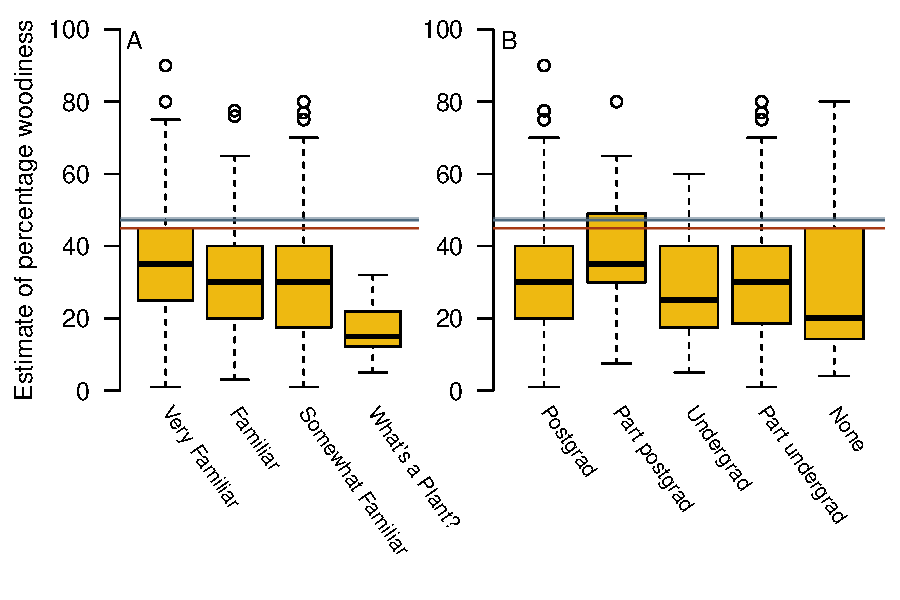
\includegraphics{figs/survey-results}
  \caption{Distribution of responses to the survey question ``What
    percentage of the world's vascular plant species are
    woody?''. Responses are broken up by familiarity with plants
    (panel (a)) and formal training in botany or a related discipline
    (panel (b)). The mean and 95\% confidence intervals for our
    estimates of the proportion of woody species from the empirical
    data are depicted by the horizontal shaded rectangles; the blue
    upper rectangle corresponds to the ``weak prior'' approach and the
    red lower rectangle corresponds to the ``strong prior'' approach
    (see Appendix for details).}
  \label{fig:survey}
\end{figure}

\begin{figure}[p]
  \centering
  \includegraphics{figs/fraction-by-genus}
  \caption{Distribution of the percentage of woodiness among genera.
    The distribution of the percentage of species that are woody within
    a genus is strongly bimodal among genera (panel a -- showing
    genera with at least 10 species only).
    % 
    The two different sampling approaches generate distributions that
    differ in their bimodality (panel b). When assuming species are
    sampled with replacement from some pool, but having no prior on
    the fraction of woodiness within the pool generates a broad
    distribution with many polymorphic genera (blue lines), while
    sampling with replacement assuming that species are drawn from a
    pool of species that has a fraction of woody species equal to the
    observed fraction of woodiness generates a strongly bimodal
    distribution (red lines).}
  \label{fig:distribution-genera}
\end{figure}

\begin{figure}[p]
  \centering
  \includegraphics{figs/fraction-on-phylogeny}
  \caption{Distribution of the percentage of woodiness among orders of
    vascular plants.  Each tip represents an order, with the width of
    the sector proportional to the log number of recognised species in
    that order (data from accepted names in ref \citep{ThePlantList}).
    The bars around the perimeter indicate the percentage of woody
    (brown) and herbaceous (green) species, estimated using the
    ``strong prior'' (sampling without replacement) approach.  Using
    the ``weak prior'' approach generally leads to an estimated
    percentage that is closer to 50\% (see Figures
    \ref{fig:phylogeny-supp} and \ref{fig:distribution-genera}).}
\label{fig:phylogeny}
\end{figure}

\clearpage
\renewcommand\thefigure{S.\arabic{figure}}
\setcounter{figure}{0}    

\begin{figure}[p]
  \centering
  \vspace{-20ex}
  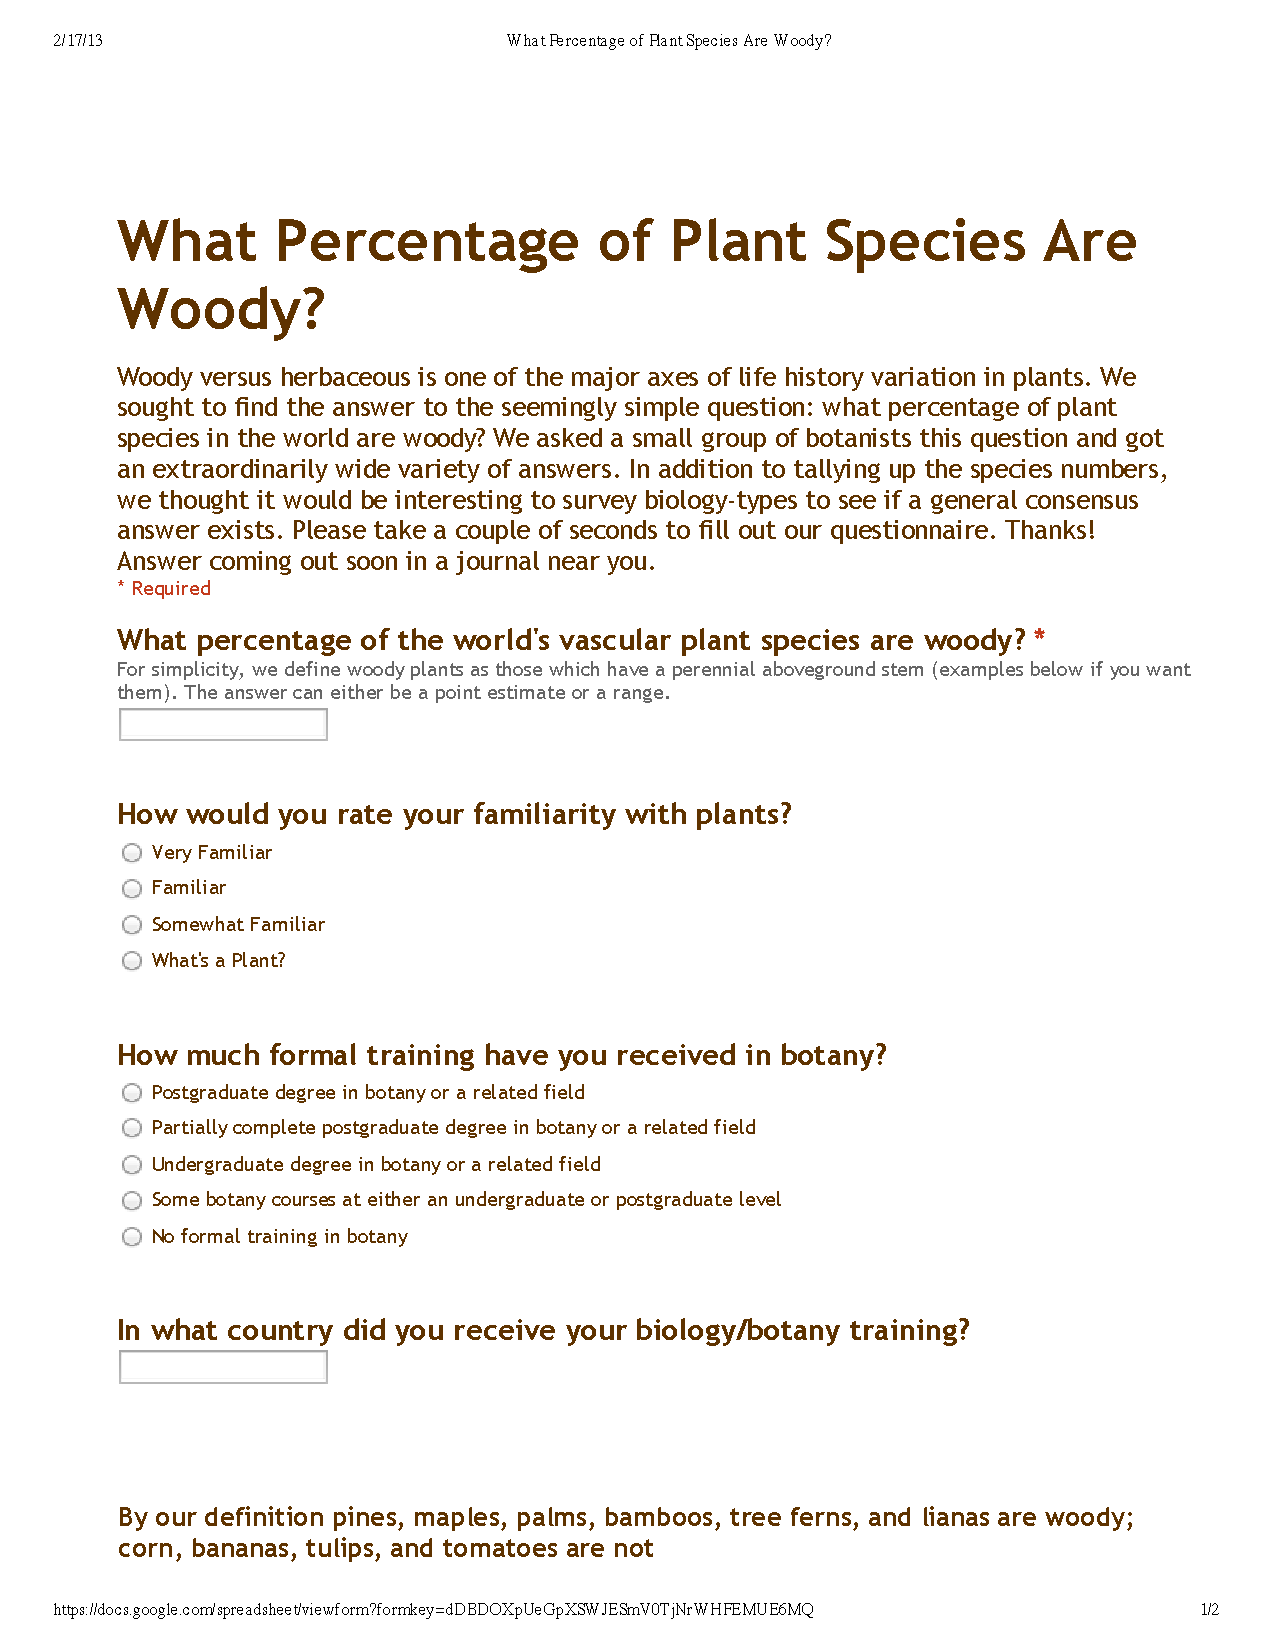
\includegraphics[scale=0.7]{figs/Survey_supplemental}
  \caption{(Supplementary) English-language version of the survey we
    distributed}
  \label{fig:survey-text}
\end{figure}

\begin{figure}[p]
  \centering
  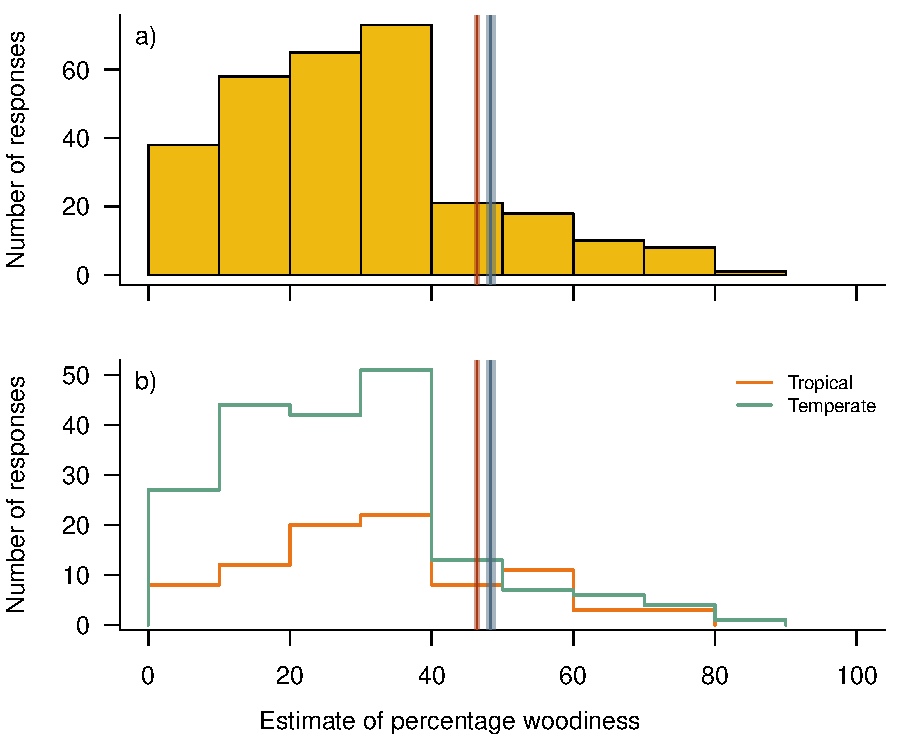
\includegraphics{figs/survey-distribution}
  \caption{(Supplementary) Distribution of all responses to the survey
    question ``What percentage of the world's vascular plant species
    are woody?''.
    %
    The mean and 95\% confidence intervals for our estimates of the
    proportion of woody species from the empirical data are depicted
    by the horizontal shaded rectangles; the blue rectangle
    corresponds to the ``weak prior'' approach and the red rectangle
    corresponds to the ``strong prior'' approach (see Appendix for
    details).  
    % 
    Panel a) includes all 292 responses.  In panel b), the 282
    responses that indicated country are shown separated into
    ``tropical'' (orange distribution) and ``temperate'' (teal).
    Estimates from tropical countries were slightly, but
    significantly, higher than those from temperate countries
    ($p=$0.02, $r^2$=0.016).
  }

  \label{fig:survey-distribution}
\end{figure}

\begin{figure}[p]
  \centering
  \includegraphics{figs/fraction-on-phylogeny-supp}

  \caption{(Supplementary)
    \textit{This is Figure \ref{fig:phylogeny} using the alternative
      sampling approach.}\\
    %
    Distribution of the fraction of woodiness among orders of vascular
    plants.  Each tip represents an order, with the fraction of
    circumference proportional to the log number of recognised species
    in that order (data from accepted names in ref
    \citep{ThePlantList}).  The bars around the perimeter indicate the
    percentage of woody (brown) and herbaceous (green) species,
    estimated using the ``weak prior'' (sampling with replacement)
    approach.  Using the ``strong prior'' approach generally leads to
    an estimated percentage that is further away from 50\% (see
    Figures \ref{fig:phylogeny} and \ref{fig:distribution-genera}).}
  \label{fig:phylogeny-supp}
\end{figure}

\begin{figure}[p]
  \centering
  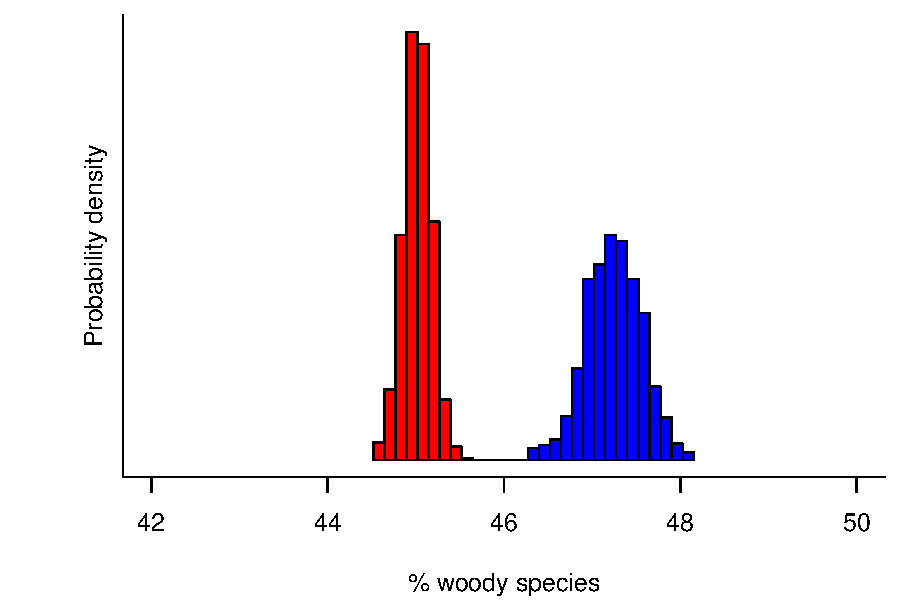
\includegraphics{figs/distribution-raw}  
  \caption{(Supplementary) The posterior probability distribution for
    the proportion of the world's flora that is woody, using our two
    sampling approaches.  The red (left) distribution samples missing species
    with replacement (strong prior), while the blue distribution
    (right) samples missing species without replacement (weak prior).
    See Appendix for details.}
  \label{fig:distribution-raw}
\end{figure}

\begin{table}[p]
  \centering
  \textit{[too large to set; see csv file]}
  \caption{Look-up table for converting the 103 growth form categories
    in the Royal Botanic Gardens Kew database into a binary
woody/herbaceous coding.}
\label{tab:kew}
\end{table}

\end{document}

%%% Local Variables:
%%% mode: latex
%%% TeX-master: t
%%% TeX-PDF-mode: t
%%% End:


